\begin{question}
\noindent Triangle $A$ has vertices $(1,1)$, $(1,3)$ and $(2,1)$, as shown on the grid below.

\begin{center}
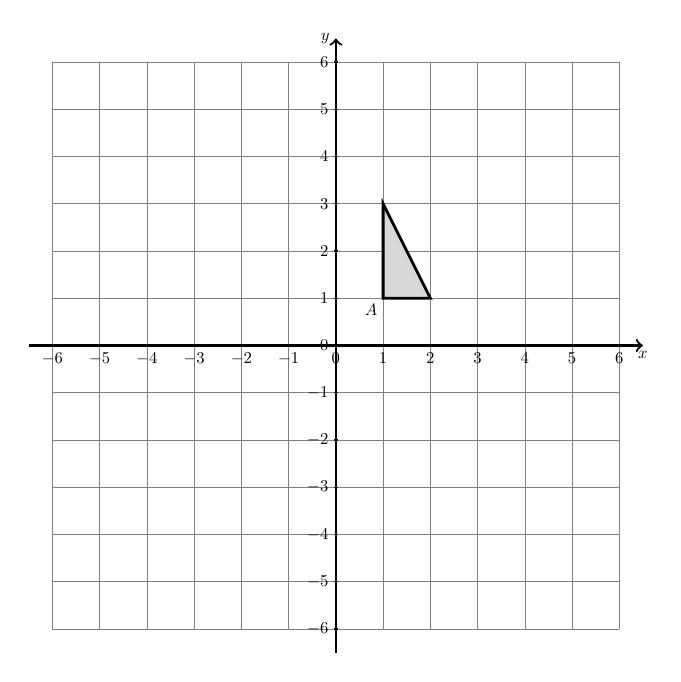
\begin{tikzpicture}[scale=0.6, transform shape]
    \def\axisLimit{6}

    \definecolor{borderColour}{HTML}{000000}
    \definecolor{fillColour}{HTML}{D8D8D8}

    % Draw grid
    \draw[step=1cm,gray,very thin] (-\axisLimit,-\axisLimit) grid (\axisLimit,\axisLimit);

    % Draw axes
    \draw[thick,->] (-\axisLimit-0.5,0) -- (\axisLimit+0.5,0) node[anchor=north] {$x$};
    \draw[thick,->] (0,-\axisLimit-0.5) -- (0,\axisLimit+0.5) node[anchor=east] {$y$};

    \foreach \x in {-\axisLimit,...,\axisLimit}
        \draw (\x cm,1pt) -- (\x cm,-1pt) node[anchor=north] {$\x$};
    \foreach \y in {-\axisLimit,...,\axisLimit}
        \draw (1pt,\y cm) -- (-1pt,\y cm) node[anchor=east] {$\y$};

    % Triangle A
    \coordinate (A1) at (1,1);
    \coordinate (A2) at (1,3);
    \coordinate (A3) at (2,1);
    \filldraw[fill=fillColour, draw=borderColour, line width=1pt] (A1) -- (A2) -- (A3) -- cycle;
    \node[below left] at (A1) {$A$};
\end{tikzpicture}
\end{center}

\begin{enumerate}
    \item[(a)] Triangle $A$ is translated by the vector $\begin{pmatrix} 2 \\ 1 \end{pmatrix}$ to give triangle $B$.

    Triangle $B$ is then reflected in the $y$-axis to give triangle $C$.

    Find the coordinates of the vertices of triangle $C$, and draw triangle $C$ on the grid above.

    \vspace{4cm}
    \answerplain{2}

    \item[(b)] Show that the single transformation that maps triangle $A$ directly onto triangle $C$ cannot be a translation.

    \vspace{4cm}
    \answerlines{4}{2}
\end{enumerate}
\end{question}
